\documentclass[10pt, landscape]{article}
\usepackage[scaled=0.92]{helvet}
\usepackage{multicol}
\usepackage{calc}
\usepackage{ifthen}
\usepackage[landscape]{geometry}
%\usepackage{hyperref}

\usepackage{newtxtext} 

%for strikeout
\usepackage{ulem}

%For editing parbox
\usepackage[table]{xcolor}
%For editing itemise margins, reduce iterm separaion and list separation
\usepackage{enumitem}
% For math
\usepackage{amsmath,amsthm,amsfonts,amssymb}

%For pictures / figures
\usepackage{color,graphicx,overpic}
\graphicspath{ {./images/} }

%\usepackage{newtxtext} 
%\usepackage{amssymb}
%\usepackage[table]{xcolor}
%\usepackage{vwcol}
%\usepackage{tikz}
%\usepackage{wrapfig}
%\usepackage{makecell}

\pdfinfo{
  /Title (CS2106-notes.pdf)
  /Creator (Ger Teck)
  /Author (Ger Teck)
  /Subject ()
  /Keywords (tex)}

%% Margins for PAPER

% This sets page margins to .5 inch if using letter paper, and to 1cm
% if using A4 paper. (This probably isn't strictly necessary.)
% If using another size paper, use default 1cm margins.
\ifthenelse{\lengthtest { \paperwidth = 11in}}
	{ \geometry{top=.3in,left=.3in,right=.3in,bottom=.3in} }
	{\ifthenelse{ \lengthtest{ \paperwidth = 297mm}}
		{\geometry{top=0.5cm,left=0.5cm,right=0.5cm,bottom=0.5cm} }
		{\geometry{top=0.5cm,left=0.5cm,right=0.5cm,bottom=0.5cm} }
	}

% Turn off header and footer
\pagestyle{empty}
% for tight centres (less spacing)
\newenvironment{tightcenter}{%
  \setlength\topsep{0.5pt}
  \setlength\parskip{0.5pt}
  \begin{center}
}{%
  \end{center}
}

% Redefine section commands to use less space
\makeatletter
\renewcommand{\section}{\@startsection{section}{1}{0mm}%
                                {-1ex plus -.5ex minus -.2ex}%
                                {0.5ex plus .2ex}%x
                                {\normalfont\large\bfseries}}
\renewcommand{\subsection}{\@startsection{subsection}{2}{0mm}%
                                {-1explus -.5ex minus -.2ex}%
                                {0.5ex plus .2ex}%
                                {\normalfont\normalsize\bfseries}}
\renewcommand{\subsubsection}{\@startsection{subsubsection}{3}{0mm}%
                                {-1ex plus -.5ex minus -.2ex}%
                                {1ex plus .2ex}%
                                {\normalfont\small\bfseries}}
% change font
%\renewcommand{\familydefault}{\sfdefault}
%\renewcommand\rmdefault{\sfdefault}
\linespread{1.05}

\makeatother

% Define BibTeX command
\def\BibTeX{{\rm B\kern-.05em{\sc i\kern-.025em b}\kern-.08em
    T\kern-.1667em\lower.7ex\hbox{E}\kern-.125emX}}

% Don't print section numbers
\setcounter{secnumdepth}{0}

\setlength{\parindent}{0pt}
\setlength{\parskip}{0pt plus 0.5ex}

%% this changes all items (enumerate and itemize, reduce margins) ITEMIZE SEPARATION HERE
\setlength{\leftmargini}{0.5cm}
\setlength{\leftmarginii}{0.5cm}
\setlist[itemize,1]{leftmargin=2mm,labelindent=1mm,labelsep=1mm, itemsep = 0mm}
\setlist[itemize,2]{leftmargin=4mm,labelindent=1mm,labelsep=1mm, itemsep = 0mm}

%itemsep = 0mm
%\setlist{nosep}

% -------------------------------------------------------------------------------

% START OF DOCUMENT HERE

\begin{document}
\raggedright
\footnotesize
\begin{multicols*}{3}

% multicol parameters
% These lengths are set only within the two main columns
%\setlength{\columnseprule}{0.25pt}
\setlength{\premulticols}{1pt}
\setlength{\postmulticols}{1pt}
\setlength{\multicolsep}{1pt}
\setlength{\columnsep}{2pt}

%% DOCUMENT NAME HERE
\begin{center}
     \Large{\textbf{CS2106 Intro Op. Systems Notes}} \\
\end{center}
AY23/24 Sem 2, github.com/gerteck


\section{1. Introduction}

\textbf{Course objectives:} Introduces basic concepts in operating systems. Focusing on OS structure and architecture, process management, memory management, file management and OS protection mechanism. At the end of the course, identify and understand major functionalities of modern operating systems and extend and apply the knowledge in future related courses.

\textbf{Supplementary Text}: Modern Operating System (5th Edition), by Andrew S. Tanenbaum, Pearson, 2023.

\subsection{Learning Outcomes}
\begin{itemize}
	\item Understand how an \textbf{OS manages computational resources for multiple users and applications, and the impact on application performance}
	\item Appreciate the \textbf{abstractions and interfaces provided by OS}
	\item Write \textbf{multi-process / thread programs} and avoid common pitfalls such as \textbf{deadlocks, starvation and race conditions.}
	\item Write system programs that utilizes \textbf{POSIX} syscall for process, memory and I/O management.
	\item Self-learn and explore advanced OS topics.
	\item Understand important design principles in complex systems.
\end{itemize}

Areas to focus on: Try to understand how things are running in parallel, since we naturally think sequentially. Secondly, how we can manage memory and how they combine and interact (in strange ways), synchronization.

\subsection{Operating System OS}
An OS is a program that acts as an intermediary between a computer user and the computer hardware. Motivation for OS:
\begin{itemize}
\item Manage resources and coordination. (Resource Allocator: Process synchronization, resource sharing)
\item Simplify programming (Abstraction of hardware / hardware virtualization, convenient services)
\item Enforce usage policies
\item Security and protection
\item User Program Portability (across different hardware)
\item Efficiency (Optimize for particular usage and hardware).
\end{itemize}

\textbf{Kernel Mode}: Complete access to all hardware resources. \\
\textbf{User Mode}: Limited / Controlled access to hardware resources.

\hspace{0.5cm}

\centerline{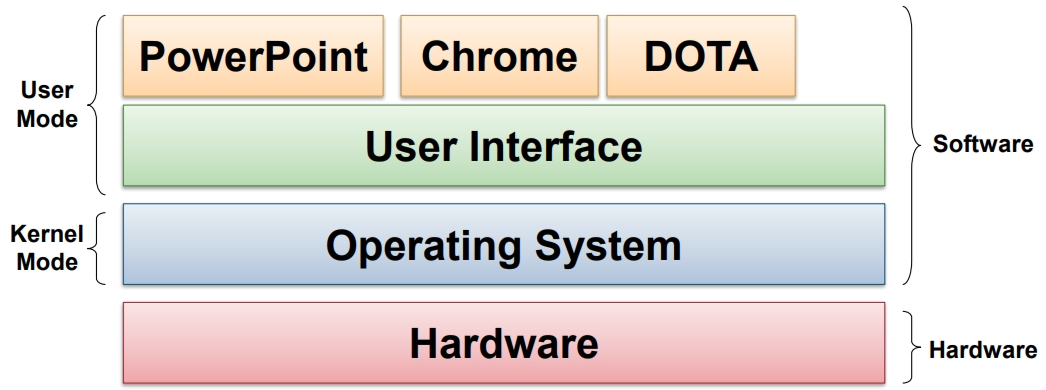
\includegraphics[width=0.5\linewidth]{highlevelOS}}

\subsubsection{Generic OS Components}
\centerline{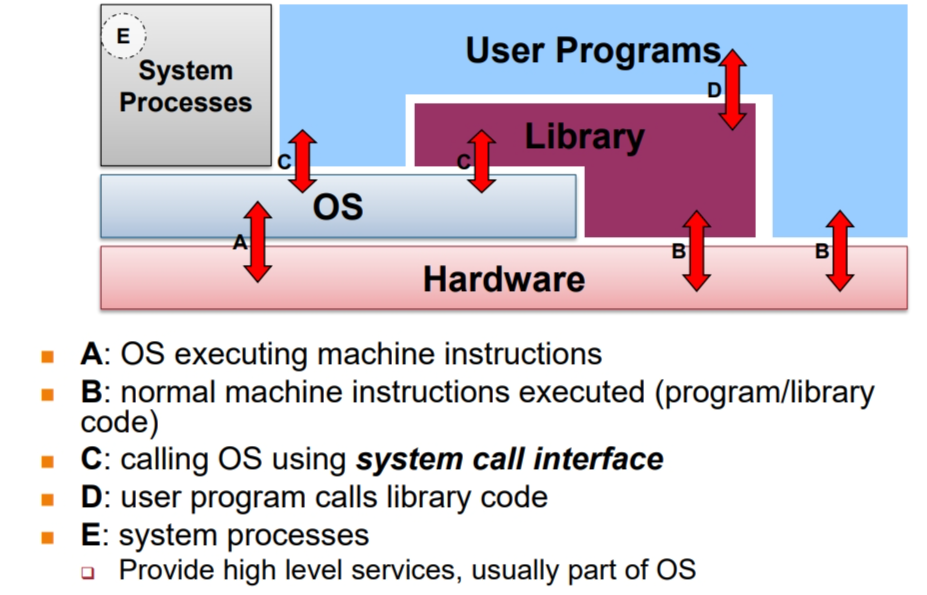
\includegraphics[width=0.7\linewidth]{genericOS}}
\begin{itemize}
\item OS is known as the \textbf{kernel}. \\
		Program that deals with hardware issues, provide system call interface and special code for interrupt handlers, device drivers.
\item Kernel code is different from normal programs: \\
		No use of system call in kernal code, can't use normal libraries, no normal I/O (must do I/O itself).
\item \textbf{Implementing OS}: Historically in assembly/machine, now in HLLs (C, C++). Heavily hardware achitecture dependent. Challenges include complexity, debugging, codebase size.
\end{itemize}

\subsubsection{OS Structures}
\textbf{Monolithic OS}: One Big program.
\begin{itemize}
\item Well understood, good performance, but highly coupled components (everything running in kernel mode) and usually devolved into very complicated internal structure.
\end{itemize}

\textbf{Microkernel OS}: 
\begin{itemize}
\item Kernel is very small and clean, only providing basic and essential facilities.
\item Inter-Process Communication \textbf{(IPC)}, Address space management, Thread management etc.
\item Higher level services are built on top of basic facilities, run as server process \textit{outside} of OS, use IPC to communicate.
\item Kernel is more robust and extendible, better isolation and protection between kernel and high level services. But, lower performance. (Latency)
\end{itemize}
\centerline{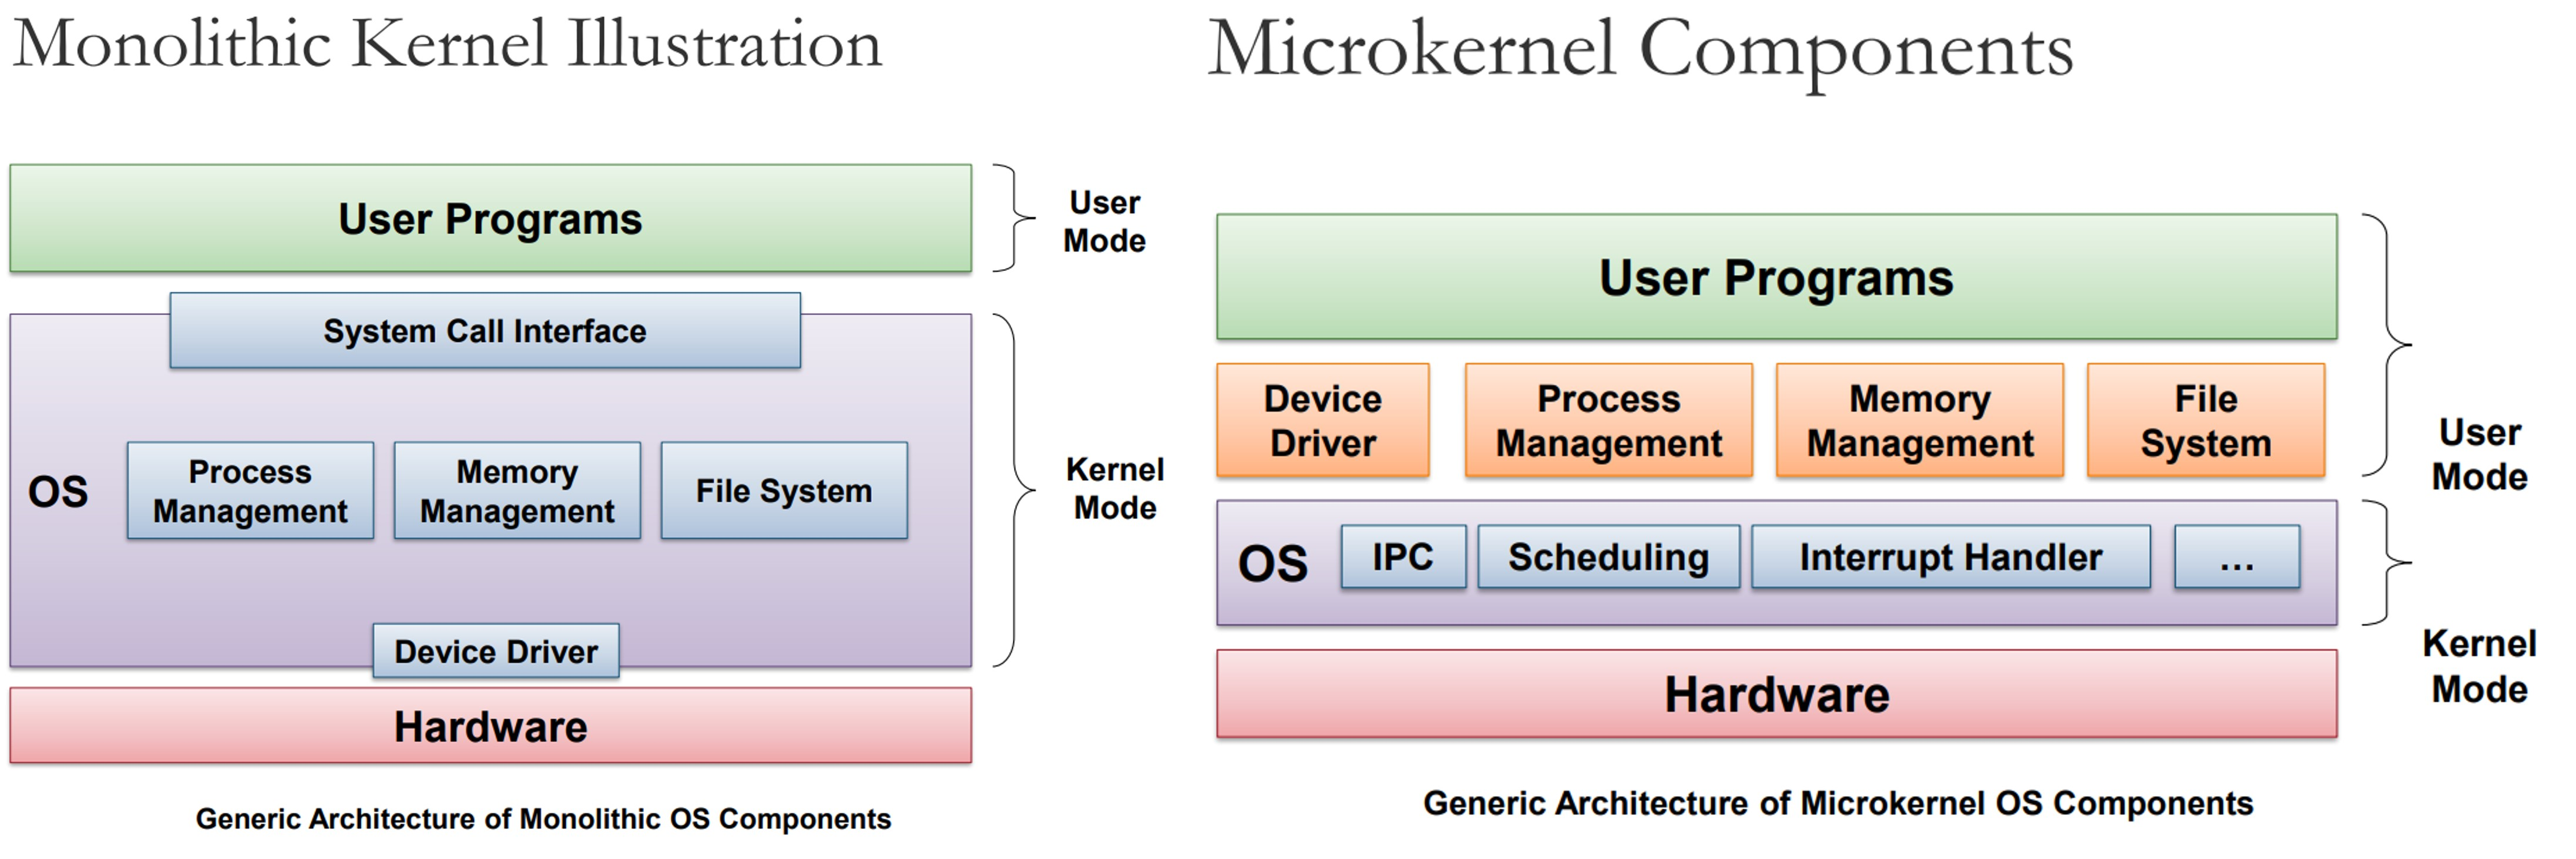
\includegraphics[width=0.95\linewidth]{OSstructure}}

\textbf{Other OS Structure}
\begin{itemize}
\item \textbf{Layered Systems}: Generalization of monolithic system, organize components into hierarchy of layers. Lowest is hardware, highest is user interface.
\item \textbf{Client-Server Model}: Variation of microkernel. Two classes of processes: Client p. request service from server process, server process built on top of microkernel. Client \& Server process can be on separate machine.
\end{itemize}







\vfill \null
\columnbreak


\section{Upcoming Topics}

\begin{itemize}
	
	\item 2. Process Abstraction
	\item 3. Process Scheduling
	\item 4. Inter-Process Communication
	\item 5. Threads + Synchronization
	\item 6. Memory Management
	\item 7. Disjoint Memory Management
	\item 8. File System Management
	\item 9. File System Implementation

\end{itemize}


~ End.





















































































\end{multicols*}
\end{document}
